\documentclass{scrartcl}
\usepackage{listings}
\usepackage{xcolor}
\usepackage{graphicx}
\usepackage{float}
\usepackage[english]{babel}
\usepackage[toc,page]{appendix}
\setlength{\topmargin}{-.5in}
\setlength{\textheight}{9in}
\setlength{\oddsidemargin}{.125in}
\setlength{\textwidth}{6in}
\def\UrlFont{\em}

\colorlet{punct}{red!60!black}
\definecolor{background}{HTML}{EEEEEE}
\definecolor{delim}{RGB}{20,105,176}
\colorlet{numb}{magenta!60!black}

\lstdefinelanguage{json}{
    basicstyle=\small\ttfamily,
    numbers=left,
    numberstyle=\scriptsize,
    stepnumber=1,
    numbersep=8pt,
    showstringspaces=false,
    breaklines=true,
    frame=lines,
    tabsize=2,
    backgroundcolor=\color{background},
    literate=
     *{0}{{{\color{numb}0}}}{1}
      {1}{{{\color{numb}1}}}{1}
      {2}{{{\color{numb}2}}}{1}
      {3}{{{\color{numb}3}}}{1}
      {4}{{{\color{numb}4}}}{1}
      {5}{{{\color{numb}5}}}{1}
      {6}{{{\color{numb}6}}}{1}
      {7}{{{\color{numb}7}}}{1}
      {8}{{{\color{numb}8}}}{1}
      {9}{{{\color{numb}9}}}{1}
      {:}{{{\color{punct}{:}}}}{1}
      {,}{{{\color{punct}{,}}}}{1}
      {\{}{{{\color{delim}{\{}}}}{1}
      {\}}{{{\color{delim}{\}}}}}{1}
      {[}{{{\color{delim}{[}}}}{1}
      {]}{{{\color{delim}{]}}}}{1},
}

\begin{document}
\author{Andreas Bjoru \& Srini Venkatesh\\ Florida Institute of Technology}
\title{CSE 5231 Computer Networks}
\subtitle{Class Project Report, Fall 2013}
\renewcommand{\today}{November 26, 2013}
\maketitle
\tableofcontents
\newpage

\section{Summary}
The objective of this project is to demonstrate the functionality of some of the OSI layers in the communication stack. In particular, key functions performed by layers 2 (Data Link), 3 (Network) and 4 (Transport) is to be emulated for the purpose of transferring a file from one network node to another \cite{assignment}. 

\section{Architecture}
The architecture of the network simulator is fairly simple. The main application class, \texttt{Simulator}, is responsible for reading the topology and creating each network node. A network node, \textit{host or router}, are represented as system threads. Each of these network nodes share a common super-class \texttt{AbstractNetworkNode} that defines common functionality and basic implementation for the OSI layer methods. The OSI layer methods shares the same pattern in which they handle both incoming and outgoing data. This is achieved through the \texttt{Transmit} enum type that is a required argument along with the data payload. \\

The \texttt{physicalLayer(byte[], Transmit, Address)} method will send a given packet to every node attached to the same network, thereby simulating the task of writing a packet on the 'wire'. This is achieved by collecting every node attached to the sender's network address through the use of utility methods on the \texttt{Topology} class. When the physical layer method receives a packet, it will just hand it off to the layer above it.\\

The \texttt{linkLayer(byte[], Transmit, Address)} method will packet a given payload in an \texttt{EthernetFrame} along with the source and destination MAC addresses from the \texttt{Address} argument. The frame will then be handed down to the physical layer method to complete the sending responsibilities of the layer. When the link layer receives a packet it will first verify the cyclic redundancy check (CRC) sum of the packet. If this check fails, the packet will be dropped. The next check performed is the destination MAC address check which determines if the packet is actually for this node. If the destination MAC address matches the network node, then the payload of the packet is handed off to the layer above it. Otherwise, the packet is simply dropped since it is not addressed for this node.

\subsection{Network hosts}
The \texttt{transport(payload, transmit, addr)} method slices payload into segments while sending and assembles the segments when it receive the payload. When sending a given payload, it slices the payload into many segments based on the payload size. First it will check the length of the payload to make sure it needs to be sliced to MTU's size or not. If the payload size is more than the MTU's size then it will slice the segments considering the header length. These segments has TCP header along with data. Source and destination ports are included in the header. SYN and FIN flags are used to identify segments starting and ending point. This payload will be sent to network layer for adding IP header and route this segment to right node. Sending parameters would be \texttt{networkLayer(byte[], Transmit, Address)} method. \\

When receiving a payload, this method will convert the payload into segments. It will then extract the chechsum to make sure segment is valid, if it's not valid it drops. If not, it keeps accumulating the segments into a buffer. along with sequence number. Then it will check for the FIN flag in the header to confirm that that's the last segment. If it's not FIN (it must be SYN), then it keeps assembling the segments to build a complete payload. Once the payload is built, it will be sent to application layer for creating a file in destination node.


\subsection{Network routers}
The functionality of the network layer is overridden for routers since they will just route packages to the next network or host. Similar to the inherited version of this method, it will start by verifying the IP header checksum. If the verification fails, the package is dropped. Otherwise, the correct network interface is found and the MAC address of that interface is used as the new source MAC address. The destination MAC address is then resolved through \texttt{Topology arpResolve(IP)},  and the payload is sent to the \texttt{linkLayer(byte[], edu.fit.cs.computernetworks.AbstractNetworkNode.Transmit, Address)} method if the router.

\subsection{Topology}
The topology for the network described by the assignment was fixed (see figure \ref{fig:topo}). In order to avoid having to hard-code information extracted from this topology (routing tables, MAC tables, etc), we decided to represent the topology in an external format as seen in appendix \ref{appendix:topology}. This will also allow us to change the topology of the network without having to change the implementation. Each node in the topology is represented by a corresponding node in the \textit{JSON} file including relevant information (see table below). Furthermore, the topology representation also contains the hardware address lookup table for the network.

\begin{center}
\begin{tabular}{l|{c}|{l}}
\textbf{Element} & \textbf{Type} & \textbf{Description} \\
\hline
id & Host, Router & Hostname for the network node \\ \hline
ip & Host & IP address for a \textit{host} \\ \hline
mask & Host & Network mask for a \textit{host} \\ \hline
mac & Host & Hardware address for a \textit{host} \\ \hline
mtu & Host & Maximum transmit unit for a \textit{host} \\ \hline
gateway & Host & Default gateway for a \textit{host} \\ \hline
routing & Host, Router & Routing table for the network node \\ \hline
ports & Router & Array of network interfaces for a \textit{router} \\ \hline
port $\to$ ip & Router & IP address for a given port on a \textit{router} \\ \hline
port $\to$ mask & Router & Network mask for a given port on a \textit{router} \\ \hline
port $\to$ mac & Router & Hardware address for a given port on a \textit{router} \\ \hline
port $\to$ mtu & Router & Maximum transmit unit for a given port on a \textit{router} \\ \hline
\end{tabular}
\end{center}

The topology representation is mapped to corresponding Java classes using a 3rd-party library called \texttt{Jackson}, which sole purpose is to process the \texttt{JSON} data format. The Java package \texttt{edu.fit.cs.computernetworks.topology} contains the mapped types which is briefly explained below.

\begin{description}
\item[Topology] is the root class of the topology model.
\item[Node] defines an abstract superclass for both Host and Router.
\item[Host] describes a network host.
\item[Router] describes a network router.
\item[Port] describes a network interface on a Router.
\item[RoutingEntry] describes an entry in a node's routing table.
\item[MACTableEntry] describes an entry in the global ARP table.
\end{description}

\section{Data flow}
Basically how data flows between network nodes. Explain how the layer methods work..

\section{Execution}
This project is built on eclipse environment with some additional packages. So first we need to download and install these packages by following the given steps.
\subsection{Windows Environment:}
1. Go to command prompt and navigate to the project's root location \\
2. Execute this command: gradlew.bat eclipse \\
3. The gradlew command is a wrapper around the gradle build tool and will download the binaries for the build tool before executing the task. \\
4. When gradle finishes (i.e. eclipse project files have been generated), you can import the project in eclipse by selecting ‘import then existing project’ from the eclipse menus. \\ 
5. Create sample folder to place the file to tansfer to different nodes.

For Example: Like, {C:\textbackslash tmp\textbackslash A}, {C:\textbackslash tmp\textbackslash B}, {C:\textbackslash tmp\textbackslash C}  \\
6. Execute the following command: 

gradlew.bat run -ProotPath=C:\textbackslash tmp
\subsection{Unix Environment:}
1. Go to command prompt and navigate to the project's root location \\ 
2. Execute this command: {gradlew eclipse} \\
3. The gradlew command is a wrapper around the gradle build tool and will download the binaries for the build tool before executing the task. \\
4. When gradle finishes (i.e. eclipse project files have been generated), you can import the project in eclipse by selecting ‘import -> existing project’ from the eclipse menus. \\
5. Create sample folder to place the file to tansfer to different nodes.

For Example: Like, /tmp/A,  /tmp/B,  /tmp/C \\
6. Execute the following command: 

gradlew run -ProotPath=/tmp \\ \\
Notice the property ‘rootPath’ that specifies the root path from where the threads will listen for files. The default path is still ‘/tmp/{id}’ where id is the name of the host node \\ \\

\section{Output}
This section contains the output of the application for different scenarios. \\

\subsection{1 KB File transfer from Node-A to Node-B (B.txt)}
\lstinputlisting[language=json,firstnumber=1]{../FromAtoB-1kb.log}
\subsection{1 KB File transfer from Node-B to Node-C (C.txt)}
\lstinputlisting[language=json,firstnumber=1]{../FromBtoC-1kb.log}
\subsection{121 KB File transfer from Node-A to Node-C (C.jpg)}
\lstinputlisting[language=json,firstnumber=1]{../FromAtoC-121kb.log}
\subsection{276 KB File transfer from Node-B to Node-A (A.gif)}
\lstinputlisting[language=json,firstnumber=1]{../FromBtoA-276kb.log}
\subsection{4 KB File transfer from Node-C to Node-B (B.xls)}
\lstinputlisting[language=json,firstnumber=1]{../FromCtoB-4kb.log}
\subsection{13 KB File transfer from Node-C to Node-A (A.pdf)}
\lstinputlisting[language=json,firstnumber=1]{../FromCtoA-13kb.log}

\newpage
\appendix
\section{Assignment Topology} \label{appending:topo-img}
\begin{figure}[H]
\centering
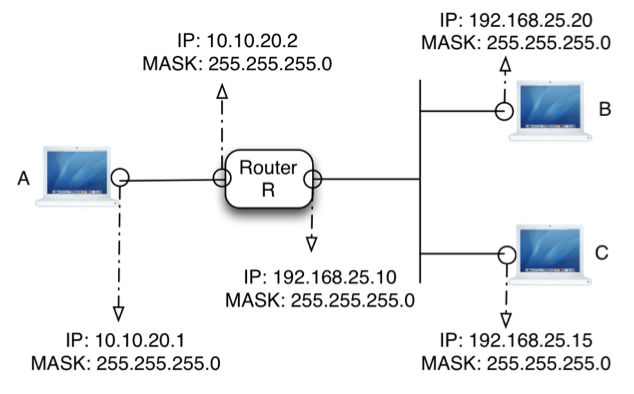
\includegraphics[scale=.65]{topology.png}
\caption{Network topology for the assignment}
\label{fig:topo}
\end{figure}
\newpage
\section{Topology Definition JSON} \label{appendix:topology}
\lstinputlisting[language=json,firstnumber=1]{../src/main/resources/topology2.json}

\newpage
%\bibliographystyle{plain}
%\bibliography{critique2}
\begin{thebibliography}{30}
\bibitem{assignment} Dr. Marco Carvalho, \emph{CSE5231 - Class Project}, Florida Institute of Technology, Fall 2013.
    
\end{thebibliography}

\end{document}